\documentclass{article}
\usepackage[german]{babel}
\usepackage{float}
\usepackage{fourier}
\usepackage[utf8]{inputenc}
\usepackage[T1]{fontenc}
\usepackage{amsfonts,amsthm, amsmath}
\usepackage{listings}
% The following is needed in order to make the code compatible
% with both latex/dvips and pdflatex.
\ifx\pdftexversion\undefined
\usepackage[dvips]{graphicx}
\else
\usepackage[pdftex]{graphicx}
\DeclareGraphicsRule{*}{mps}{*}{}
\fi

\setlength\parindent{0pt}
\lstset{language=Erlang}

\begin{document}

\textbf{Team:} TEAM 01, Falco Winkler (FW), Daniel Schruhl (DS)\\
\\
\textbf{Aufgabenteilung:}
\begin{itemize}
    \item Starter (DS)
    \item Koordinator (FW)
    \item ggT (DS,FW)
\end{itemize}

\textbf{Quellenangaben:}
\begin{itemize}
    \item Aufgabe 2, 25.04.2017, C.Klauck: \newline
    http://users.informatik.haw-hamburg.de/~klauck/VerteilteSysteme/aufg2.html
\end{itemize}

\textbf{Bearbeitungszeitraum:}
\begin{itemize}
	\item 13.04.2017 3h (FW)
	\item 24.04.2017 3h (DS)
	\item 25.04.2017 4h (DS)
	\item 26.04.2017 5h (DS, FW)
	\item 05.05.2017 2h (DS, FW)
\end{itemize}

\textbf{Aktueller Stand:}
\begin{itemize}
	\item Starter-Modul fertig und getestet
	\item ggT-Modul fertig ung getestet
	\item Koordinator-Modul fertig
\end{itemize}

\textbf{Änderung des Entwurfs:}
\begin{itemize}
    \item Keine Änderungen
\end{itemize}

\newpage

\section{Einführung und Ziele}
Mit dem Satz von Euklid ist es möglich, den größten gemeinsamen Teiler (ggT) zweier positiver ganzer Zahlen
($x,y \in \mathbb{Z}^{*}_{+}$) zu bestimmen (Gleichung \ref{equ:ggt-simple}).

Dabei wird der größte gemeinsame Teiler von $x$ und $y$ auf den größten gemeinsamen Teiler von $y$ und $\bmod{(x,y)}$
zurückgeführt.

\begin{equation}
\forall x,y \in \mathbb{Z}^{*}_{+}: ggT(x,y) = ggT(y,\bmod{(x,y)})
\label{equ:ggt-simple}
\end{equation}

Das erlaubt eine rekursive Berechnung des größten gemeinsamen Teilers.

Das Produkt soll diesen Algorithmus verteilt ausführen, verwalten und koordinieren, um den größten gemeinsamen Teiler
mehrerer verschiedener Zahlen zu berechnen.

\subsection{Randbedingungen}
Um den ggT verteilt mit dem Algorithmus berechnen zu können, muss der Algorithmus angepasst werden
(Gleichung \ref{equ:ggt-distributed}). Das ermöglicht ein Terminieren in jedem ggT-Prozess mit dem ggT und nicht mit 0,
da bei $ggT(x,x)$ terminiert wird.

\begin{multline}
\forall x,y \in \mathbb{Z}^{*}_{+}: ggT(x,y) = ggT(y,\bmod{^{*}(x,y)})\\
\bmod{^{*}(x,y)} := \bmod{(x-1, y)} + 1
\label{equ:ggt-distributed}
\end{multline}

\subsection{Kontextbegrenzung}
Das System soll in Erlang umgesetzt werden. Es muss auf Computern mit Linux Betriebssystem lauffähig sein.

\newpage

\section{Gesamtsystem}

\subsection{Bausteinsicht}
\begin{figure}[H]
    \centering
    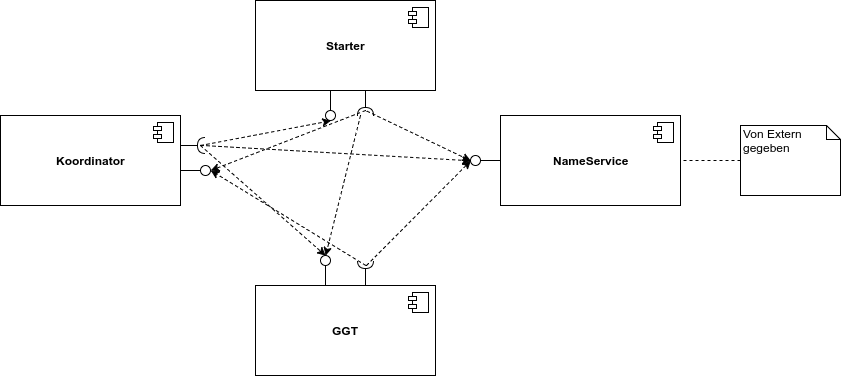
\includegraphics[width=0.5\textwidth]{component-diagram.png}
    \caption[seq-dia]{Komponentendiagramm der ggT-App}
    \label{fig:component-diagram}
\end{figure}

\subsection{Laufzeitsicht}
\begin{figure}[H]
    \centering
    \includegraphics[width=1.0\textwidth]{sequence-diagram.png}
    \caption[seq-dia]{Eine ggT Berechnung mit Abbruch per Voting}
    \label{fig:seq-diagram}
\end{figure}

\newpage

\section{Subsysteme und Komponenten}

\subsection{Starter-Modul}
\subsubsection{Aufgabe und Verantwortung}
Der Starter steht zwischen Koordinator und ggT-Prozess. Er startet mehrere ggT-Prozesse mit den Initialisierungsdaten,
die vom Koordinator zur Verfügung gestellt werden (asynchron) und seinen konfigurierbaren Parametern.

\subsubsection{Schnittstelle}
\begin{lstlisting}
/* Nachricht zum Starten von ggT-Prozessen */
{steeringval,ArbeitsZeit,TermZeit,Quota,GGTProzessnummer}

/* Startet einen Starter Prozess */
start(StarterID): Integer -> PID
\end{lstlisting}
\{\textbf{steeringval},ArbeitsZeit,TermZeit,Quota,GGTProzessnummer\}:\\
Einkommende Nachricht zum Starten von ggT
Prozessen. Die ArbeitsZeit ist die simulierte Verzögerungszeit zur Berechnung in Sekunden, die TermZeit ist die
Wartezeit in Sekunden, bis eine Wahl für eine Terminierung initiiert wird, Quota ist die konkrete Anzahl an
benötigten Zustimmungen zu einer Terminierungsabstimmung und GGTProzessnummer ist die Anzahl der zu startenden
ggT-Prozesse.\\

\textbf{start(}StarterID\textbf{)}:\\
Startet den Starter mit der gegebenen eindeutigen Nummer.\\

\subsubsection{Entwurfsentscheidungen}
Der Starter ruft in seiner Initalisierungsphase an der Schnittstelle vom Koordinator seine benötigten Parameter zum
Starten von ggT-Prozessen asynchron ab. Zusätzlich werden noch die konfigurierbaren Parameter geladen. Mit diesen Daten
werden dann die ggT-Prozesse gestartet. Die Anzahl der zu startenden ggT-Prozesse wird durch die GGTProzessnummer in der
Schnittstelle definiert.

\subsubsection{Konfigurationsparameter}
\begin{itemize}
    \item Praktikumsgruppe
    \item Teamnummer
    \item Nameservicenode definiert den Node des Nameservices
    \item Nameservicename definiert den Namen des registrierten Nameservices auf dem Nameservicenode
    \item Koordinatorname definiert den Namen des Koordinators
\end{itemize}

\newpage

\subsection{ggT-Modul}
\subsubsection{Aufgabe und Verantwortung}
Berechnung des ggTs mit dem Algorithmus verteilt auf mehrere Prozesse.

\subsubsection{Schnittstelle}
\begin{lstlisting}
/* Einkommende Nachricht zum Setzen der Namen der Nachbarn */
{setneighbors,LeftN,RightN}

/* Einkommende Nachricht zum Setzen der von diesem Prozess */
/* zu berabeitenden Zahl fuer eine neue Berechnung */
{setpm,MiNeu}

/* Einkommende Nachricht zum Senden des rekursiven Aufrufes der ggT Berechnung */
{sendy,Y}

/* Einkommende Wahlnachricht fuer die Terminierung der aktuellen Berechnung */
{From,{vote,Initiator}}

/* Einkommende Erhaltenes Abstimmungsergebnis */
{voteYes,Name}

/* Einkommende Nachricht zum Senden des aktuellen Mis an From */
{From,tellmi}

/* Einkommende Nachricht zum Senden eines pongGGT an From */
{From,pingGGT}

/* Einkommende Nachricht zum Beenden des ggT-Prozesses */
kill

/* Funktion, die einen ggT-Prozess startet */
start(WorkingTime, TerminationTime, Quota, GGTName, Coordinator, NameService):
Integer X Integer X Integer X Atom X Tupel X PID -> PID
\end{lstlisting}
\{\textbf{setneighbors},LeftN,RightN\}: Setzt die Nachbarn. LeftN und RightN sind dabei Namen, die im NameService
(und lokal im Node) registriert sind.\\

\{From,\{\textbf{vote},Initiator\}\}: Wahlnachricht für die Terminierung der aktuellen Berechnung. Der Initiator ist der
Initiator dieser Wahl (Name des ggT-Prozesses, keine PID!) und From (ist PID) ist sein Absender.\\

\{\textbf{voteYes},Name\}: Erhaltenes Abstimmungsergebnis, wobei Name der Name des Absenders ist (keine PID!).\\

\{From,\textbf{tellmi}\}: Sendet das aktuelle Mi an From (ist PID): From ! \{mi,Mi\}. Wird vom Koordinator z.B. genutzt,
um bei einem Berechnungsstillstand die Mi-Situation im Ring anzuzeigen.\\

\{From,\textbf{pingGGT}\}: Sendet ein pongGGT an From (ist PID): From ! \{pongGGT,GGTname\}. Wird vom Koordinator z.B.
genutzt, um auf manuelle Anforderung hin die Lebendigkeit des Rings zu prüfen.\\


\textbf{start(}WorkingTime, TerminationTime, Quota, GGTName, Coordinator, NameService\textbf{)}: Startet einen
ggT-Prozess mit den gegebenen Parametern. Der GGTName setzt sich zusammen aus <PraktikumsgruppenID><TeamID><Nummer des ggT-Prozess><Nummer des Starters>.
Die WorkingTime beschreibt einen simulierten Arbeitsaufwand für die Berechnung und die TerminationTime beschreibt die
Zeit, nach der ein ggT-Prozess eine Terminierungsabstimmung durchführt. Die Quota ist die konkrete Anzahl an
notwendigen Zustimmungen zu einer Terminierungsabstimmung. Coordinator und NameService sind Referenzen für die
jeweiligen Dienste.\\

\subsubsection{Entwurfsentscheidungen}
Das Modul hält sich seinen State mit einer Map. In dieser Map sind alle benötigten Variablen für den Algorithmus
und für den Betrieb des ggT-Moduls gespeichert (Config). Außerdem sind im State die Zahl Mi, der Zeitstempel der letzten
 Änderung von Mi, die Nachbarn, ein Flag für die Terminierung und die Anzahl der empfangenen yesVotes gespeichert.

Jeder Prozess Pi hat seine eigene Variable Mi, in der die von ihm zu verwaltende Zahl steht. Diese Variable Mi kann
jederzeit von außen verändert werden.
Alle Prozesse sind in einem Ring angeordnet.\\

Der ggT aller am Anfang bestehender Mi wird wie folgt berechnet:
\begin{lstlisting}
  {Eine Nachricht <y> ist eingetroffen}
  if y < Mi
    then Mi := mod(Mi-1,y)+1;
         send #Mi to all neighbours;
         send #Mi,#Time,#Name to coordinator;
  fi
\end{lstlisting}
Eine Terminierung wird eingeleitet, wenn die Termzeit abläuft und noch keine Terminierung gesendet wurde (Terminating
Flag). Die Termzeit und das Flag für Terminating wird zurückgesetzt, wenn einer Zahl empfangen wird.

Wenn ein ggT-Prozess eine Terminierung einleitet, wird ein multicast an den Nameservice gesendet. Dabei wird die Anzahl
der empfangenen Votes im State auf 0 gesetzt. An alle ggT-Prozesse wird dann ein vote vom Nameservice gesendet (siehe
Abbildung \ref{fig:seq-diagram}).

Es darf vom ggT-Prozess nur genau eine Terminierung zur Zeit eingeleitet werden. Weitere können vom Prozess frühstens
dann gestartet werden, wenn zwischenzeitlich eine Zahl (sendy, setpm) an ihn gesendet wurde. Das wird über ein Flag im
State des ggT-Prozesses geregelt.

Ist dabei seit dem letzten Empfang einer Zahl mehr als Termzeit/2 Sekunden vergangen, dann antwortet er dem Initiator
mit voteYes (explizites Zustimmen). Sonst ignoriert er die Nachricht (implizites ablehnen). Der Initiator zählt alle
einkommenden voteYes Nachrichten (im State).

Wenn dabei die Anzahl der eingetroffenen voteYes größer gleich der Quota ist, wird der Terminierungsprozess beim
Koordinator eingeleitet.
\newpage

\subsection{Koordinator-Modul}
\subsubsection{Aufgabe und Verantwortung}
Der Koordinator verwaltet alle ggT Prozesse und ordnet sie in einem Ring an, und startet die Berechnung.
Er stellt Konfigurationsparameter für Starter-Prozesse bereit. Außerdem koordiniert er die Terminierung des
gesamten Systems auf Befehl eines ggt-Prozesses oder des Nutzers.

\subsubsection{Schnittstelle}
\begin{lstlisting}
/* Einkommende Nachricht zur Anfrage nach den steuernden Werten */
/* Sendet Werte zurueck an From */
{From,getsteeringval}

/* Einkommende Nachricht zur Registrierung von ggT-Prozessen */
{hello,Clientname}

/* Einkommende Nachricht vom ggT-Prozess mit neuem Mi vom ggT-Prozess */
{briefmi,{Clientname,CMi,CZeit}}

/* Einkommende Nachricht, die das Beenden der Berechnung signalisiert. */
/* CMi und CZeit signalisieren das Ergebnis und die Uhrzeit der Terminierung */
{From,briefterm,{Clientname,CMi,CZeit}}

/* Einkommende Nachricht zum beenden aller ggT-Prozessen und setzt */
/* den Zustand auf Initialisierungsphase. */
reset

/* Zustandsuebergang Nachricht fuer Initialphase -> Arbeitsphase. */
step

/* Einkommende Nachricht zum loggen der Mis der ggT-Prozesse. */
prompt

/* Einkommende Nachricht zum loggen der Lebenszustaende der ggT-Prozesse. */
nudge

/* Wechselt das Flag zur Korrektur bei falschen Terminierungsmeldungen. */
toggle

/* Einkommende Nachricht zum Starten einer neuen ggT-Berechnung */
/* mit Wunsch-ggT WggT */
{calc,WggT}

/* Einkommende Nachricht zum Beenden des Koordinator */
/* und aller verbundenen ggT-Prozesse */
kill
\end{lstlisting}

\subsubsection{Entwurfsentscheidungen}
Im Koordinator - Modul werden die drei Zustände realisiert. Das sind die Initialisierungsphase, die Arbeitsphase und
die Beendigungsphase. In seinem State speichert er sich die kleinste empfangene Zahl von den ggT-Prozessen, eine Liste
der registrierten ggT-Prozessen und seine Config.

Die Schnittstellen der möglichen Nachrichten verändert sich je nach Zustand (durch drei receive - Schleifen).

Alle registrierten ggT-Prozesse werden im State des Koordinators mit ihrem Namen gespeichert.\\

Um den Ring zu bauen, werden die ggT-Prozesse im State gemischt und dann in einem Ring angeordnet. Dabei können sich
ab diesem Punkt keine neuen ggT-Prozesse mehr anmelden und auch keine Auskunft über die Parameter mehr gegeben werden.

Danach wird der Zustand von Bereit auf Arbeiten gewechselt. In diesem Zustand kann dann der Berechnungsvorgang für eine
feste Anzahl an Zahlen für ein Wunsch ggT und eine feste Anzahl an ggT Prozessen angestoßen werden (calc).

Der Koordinator wählt dann per Zufall 20\% aller ggT-Prozesse aus, denen er zum Start der Berechnung eine Zahl per sendy
sendet. Dabei erzeugt er für jeden der zufällig gewählten ggT-Prozessen eine Zahl (mit Wunsch ggT), die gesendet wird.\\

Um in den Zustand Beenden zu wechseln, kann dem Koordinator dieser Übergang explizit mit \textbf{kill} mitgeteilt werden.
Dann werden alle ggT-Prozesse und danach der Koordinator heruntergefahren.

Der Koordinator kann auch in den Beenden Zustand wechseln, wenn er von einem ggT-Prozess die Nachricht \textbf{briefterm}
empfängt (siehe Schnittstelle).

Falls die Korrektur der Terminierungsnachrichten (\textbf{briefterm}) aktiviert ist, wird eine Terminierungsnachricht
anhand des gesendeten Mis und der gespeicherten kleinsten empfangenen Zahl im State des Koordinators validiert.

Wenn die gesendete Zahl der Terminierung größer als die gespeicherte kleinste Zahl ist, wird eine Fehlermeldung geloggt
und die gespeicherte kleinste Zahl aus dem State dem ggT-Prozess per sendy gesendet.

Das Senden der kleinsten Zahl passiert bei deaktivierter Korrektur nicht.

\subsubsection{Konfigurationsparameter}
\begin{itemize}
    \item arbeitszeit, simulierte Verzögerungszeit zur Berechnung in Sekunden
    \item termzeit, Wartezeit in Sekunden, bis eine Wahl für eine Terminierung initiiert wird
    \item ggtprozessnummer, Anzahl der ggT-Prozesse
    \item nameservicenode, Nameservice Node
    \item nameservicename, Nameservice Name
    \item koordinatorname, Koordinator Name für den Nameservice
    \item quote, Quota, die überschritten werden muss für die Terminierungsabstimmung in Prozent
    \item korrigieren, Flag für die Korrektur der Terminierung (1/0)
\end{itemize}

\end{document}